\documentclass{exam}

\usepackage[dvipsnames]{xcolor}
\usepackage{amsmath}
\usepackage{amsfonts}
\usepackage{amsthm}
\usepackage{microtype}
\usepackage{siunitx}
\DeclareSIUnit\year{yr}
\usepackage{pgfplots}
\usepackage{graphicx}
\usepackage{sidecap}
\sidecaptionvpos{figure}{c}
\usepackage{float}
\usepackage{gensymb}
\usepackage{tkz-euclide}
\usetkzobj{all}
\usepackage{commath}
\usepackage{hyperref}

\newtheorem*{thm}{Theorem}

% russian integral
\usepackage{scalerel}
\DeclareMathOperator*{\rint}{\scalerel*{\rotatebox{17}{$\!\int\!$}}{\int}}

% \qformat{Question \thequestion: \thequestiontitle\hfill}

\begin{document}

\section*{NCEA Level 1 Mathematics (Algebra)}

\subsection*{Reading}
The second question in the homework for this week surrounds an expression that I would call \textbf{symmetric}; because of this, I thought
that I should probably provide a bit of context regarding this idea within mathematics.

A symmetry in mathematics has a formal definition, but the best way to think about it is that an object, a construction, or a concept is symmetric
if there is something that one can do to it (be it rotating it, swapping parts around in a nice manner, or some other structured action) that leaves
the object looking essentially the same.

In Q2 below, we could swap any two variables and end up with the negative of the expression. Starting with $ (a - b)(b - c)(c - a) $, we can (for
example) swap $ a $ and $ b $; we end up with $ (b - a)(a - c)(c - b) = -(a - b) \times -(c - a) \times -(b - c) = -(a-b)(b-c)(c-a) $.

Some more examples of symmetry:

\begin{center}
  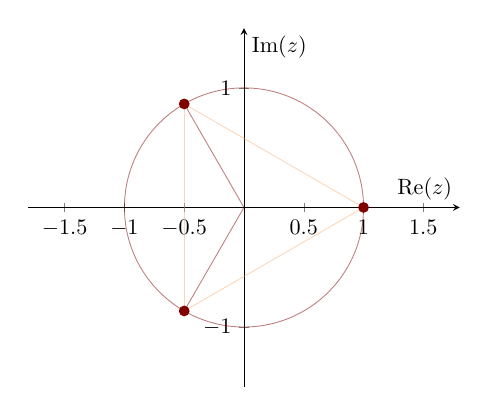
\begin{tikzpicture}[scale=0.8]
    \begin{axis}[
      xlabel=$\text{Re}(z)$,
      ylabel={$\text{Im}(z)$},
      axis lines=middle,
      disabledatascaling,
      xmin=-1.5,
      xmax=1.5,
      ymin=-1.5,
      ymax=1.5,
      axis equal
    ]
      \addplot[color=Maroon, mark=*, thick]
      coordinates {
        (1, 0)
      };
      \addplot[color=Maroon, mark=*, thick]
      coordinates {
        (-0.5, 0.866)
      };
      \addplot[color=Maroon, mark=*, thick]
      coordinates {
        (-0.5, -0.866)
      };
    \path [draw=Maroon, fill=none, semitransparent] (0,0) circle (1);
    \path [draw=Maroon, fill=none, semitransparent] (-0.5,0.866) -- (0,0);
    \path [draw=Maroon, fill=none, semitransparent] (-0.5,-0.866) -- (0,0);
    \path [draw=Apricot, fill=none, semitransparent] (-0.5,-0.866) -- (-0.5,0.866);
    \path [draw=Apricot, fill=none, semitransparent] (1, 0) -- (-0.5,0.866);
    \path [draw=Apricot, fill=none, semitransparent] (-0.5,-0.866) -- (1, 0);
    \end{axis}
  \end{tikzpicture}\\%
  \small{The three solutions to $ 1 = x^3 $ (marked with dots) are symmetric under rotation and reflection.}
\end{center}

\begin{center}
  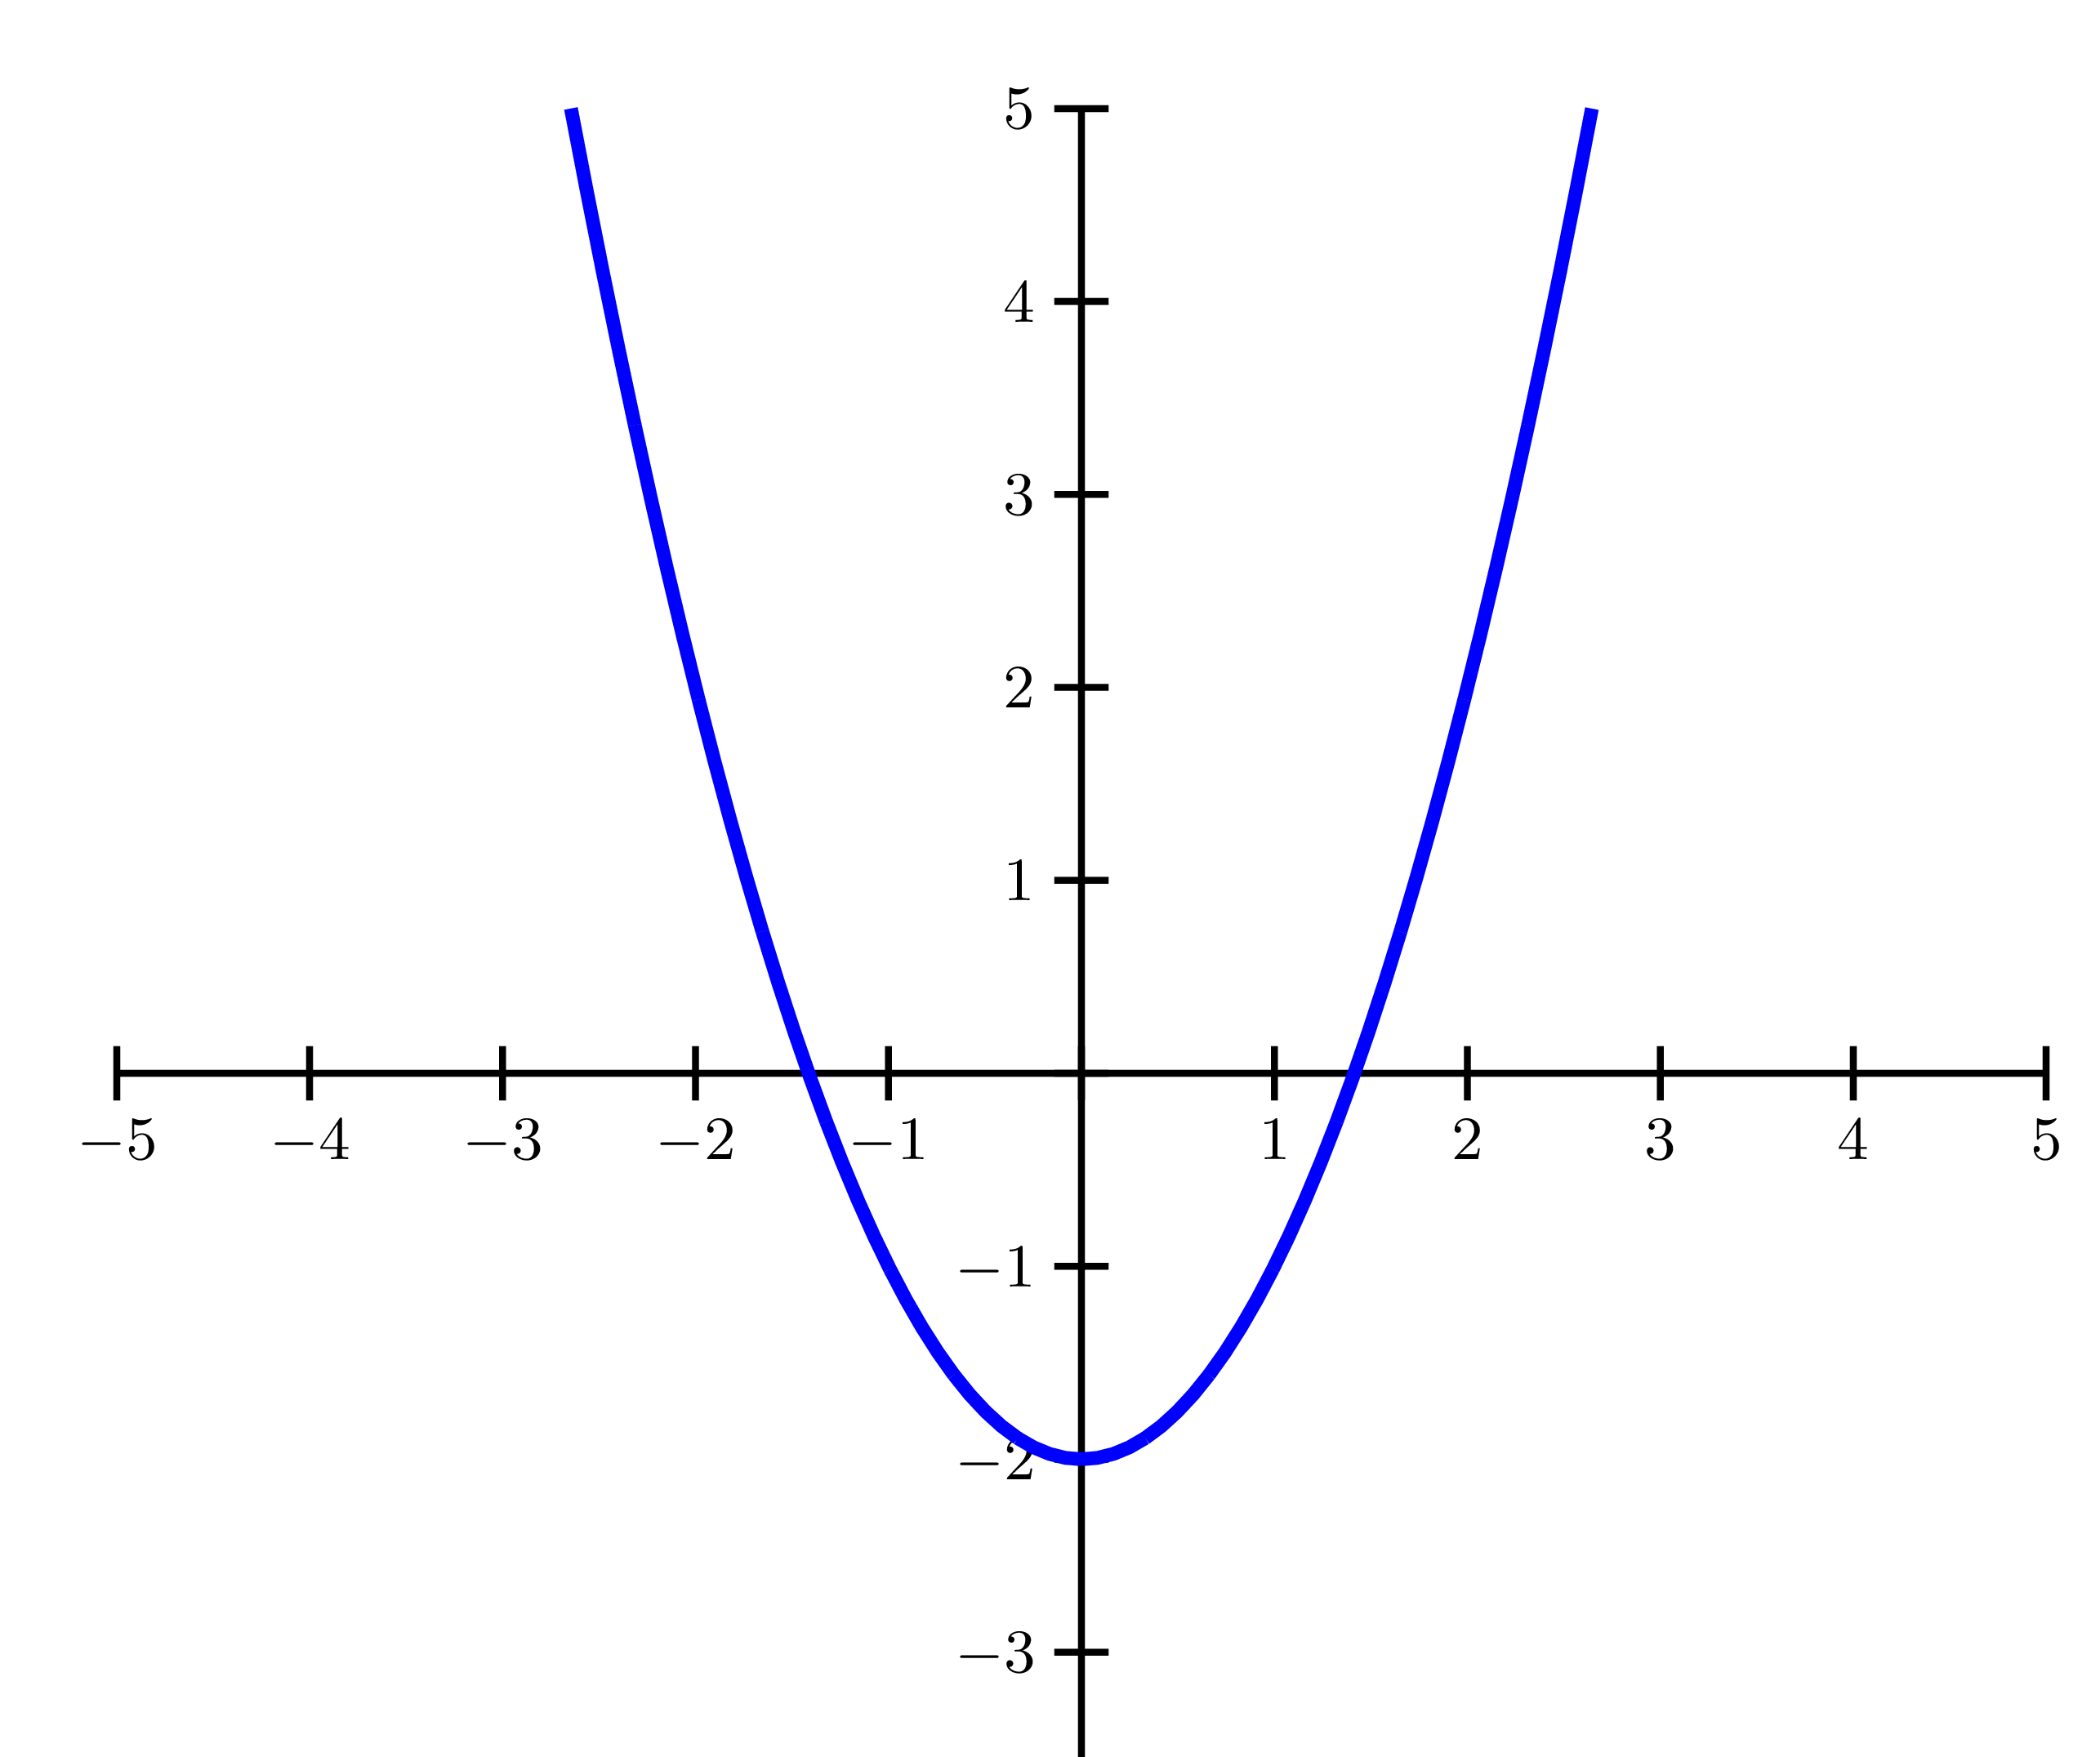
\includegraphics[width=0.3\textwidth]{parabola}
  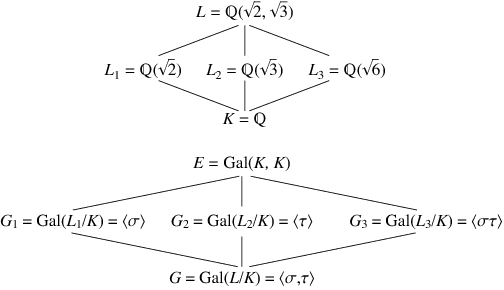
\includegraphics[width=0.3\textwidth]{galois}
  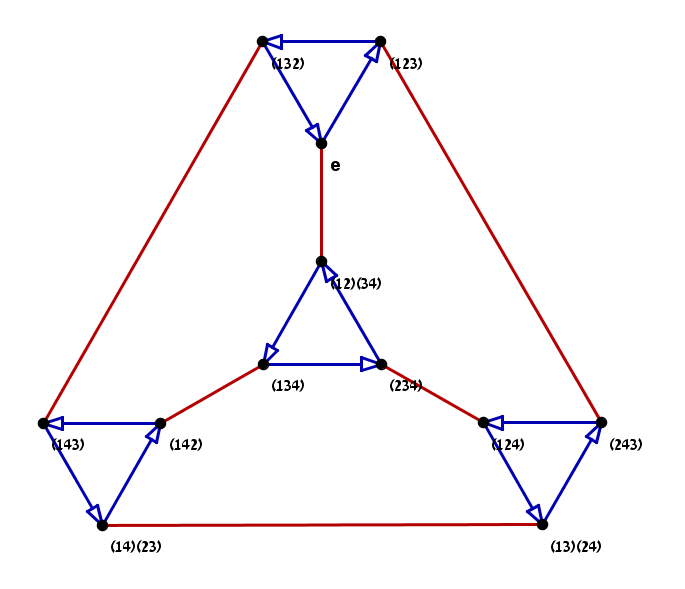
\includegraphics[width=0.3\textwidth]{cayley}\\
  \small{Left: parabola, symmetric under reflection.\\
         Centre: the top graph corresponds in some (complicated) sense to the bottom one.\\
         Right: The Cayley diagram of the group $ A_4 $ graphically displays a set of symmetries of a particular object.}
\end{center}

\subsection*{Questions}
\begin{questions}

  \question Show that $ \frac{(a - b)c + (a - b)d}{a(c + d)} = 1 - \frac{b}{a} $.
  \question Consider the expression
    \begin{equation}
      (a - b)(b - c)(c - a) \tag{*}.
    \end{equation}
    \begin{parts}
      \part Show that expression (*) is equal to $ a^2(c - b) + b^2(a - c) + c^2(b - a) $.
      \part Prove that (*) is always even, no matter what integers we choose for $ a $, $ b $, and $ c $.
    \end{parts}

\end{questions}
\end{document}
